% Options for packages loaded elsewhere
\PassOptionsToPackage{unicode}{hyperref}
\PassOptionsToPackage{hyphens}{url}
%
\documentclass[
]{article}
\usepackage{amsmath,amssymb}
\usepackage{iftex}
\ifPDFTeX
  \usepackage[T1]{fontenc}
  \usepackage[utf8]{inputenc}
  \usepackage{textcomp} % provide euro and other symbols
\else % if luatex or xetex
  \usepackage{unicode-math} % this also loads fontspec
  \defaultfontfeatures{Scale=MatchLowercase}
  \defaultfontfeatures[\rmfamily]{Ligatures=TeX,Scale=1}
\fi
\usepackage{lmodern}
\ifPDFTeX\else
  % xetex/luatex font selection
\fi
% Use upquote if available, for straight quotes in verbatim environments
\IfFileExists{upquote.sty}{\usepackage{upquote}}{}
\IfFileExists{microtype.sty}{% use microtype if available
  \usepackage[]{microtype}
  \UseMicrotypeSet[protrusion]{basicmath} % disable protrusion for tt fonts
}{}
\makeatletter
\@ifundefined{KOMAClassName}{% if non-KOMA class
  \IfFileExists{parskip.sty}{%
    \usepackage{parskip}
  }{% else
    \setlength{\parindent}{0pt}
    \setlength{\parskip}{6pt plus 2pt minus 1pt}}
}{% if KOMA class
  \KOMAoptions{parskip=half}}
\makeatother
\usepackage{xcolor}
\usepackage[margin=1in]{geometry}
\usepackage{color}
\usepackage{fancyvrb}
\newcommand{\VerbBar}{|}
\newcommand{\VERB}{\Verb[commandchars=\\\{\}]}
\DefineVerbatimEnvironment{Highlighting}{Verbatim}{commandchars=\\\{\}}
% Add ',fontsize=\small' for more characters per line
\usepackage{framed}
\definecolor{shadecolor}{RGB}{248,248,248}
\newenvironment{Shaded}{\begin{snugshade}}{\end{snugshade}}
\newcommand{\AlertTok}[1]{\textcolor[rgb]{0.94,0.16,0.16}{#1}}
\newcommand{\AnnotationTok}[1]{\textcolor[rgb]{0.56,0.35,0.01}{\textbf{\textit{#1}}}}
\newcommand{\AttributeTok}[1]{\textcolor[rgb]{0.13,0.29,0.53}{#1}}
\newcommand{\BaseNTok}[1]{\textcolor[rgb]{0.00,0.00,0.81}{#1}}
\newcommand{\BuiltInTok}[1]{#1}
\newcommand{\CharTok}[1]{\textcolor[rgb]{0.31,0.60,0.02}{#1}}
\newcommand{\CommentTok}[1]{\textcolor[rgb]{0.56,0.35,0.01}{\textit{#1}}}
\newcommand{\CommentVarTok}[1]{\textcolor[rgb]{0.56,0.35,0.01}{\textbf{\textit{#1}}}}
\newcommand{\ConstantTok}[1]{\textcolor[rgb]{0.56,0.35,0.01}{#1}}
\newcommand{\ControlFlowTok}[1]{\textcolor[rgb]{0.13,0.29,0.53}{\textbf{#1}}}
\newcommand{\DataTypeTok}[1]{\textcolor[rgb]{0.13,0.29,0.53}{#1}}
\newcommand{\DecValTok}[1]{\textcolor[rgb]{0.00,0.00,0.81}{#1}}
\newcommand{\DocumentationTok}[1]{\textcolor[rgb]{0.56,0.35,0.01}{\textbf{\textit{#1}}}}
\newcommand{\ErrorTok}[1]{\textcolor[rgb]{0.64,0.00,0.00}{\textbf{#1}}}
\newcommand{\ExtensionTok}[1]{#1}
\newcommand{\FloatTok}[1]{\textcolor[rgb]{0.00,0.00,0.81}{#1}}
\newcommand{\FunctionTok}[1]{\textcolor[rgb]{0.13,0.29,0.53}{\textbf{#1}}}
\newcommand{\ImportTok}[1]{#1}
\newcommand{\InformationTok}[1]{\textcolor[rgb]{0.56,0.35,0.01}{\textbf{\textit{#1}}}}
\newcommand{\KeywordTok}[1]{\textcolor[rgb]{0.13,0.29,0.53}{\textbf{#1}}}
\newcommand{\NormalTok}[1]{#1}
\newcommand{\OperatorTok}[1]{\textcolor[rgb]{0.81,0.36,0.00}{\textbf{#1}}}
\newcommand{\OtherTok}[1]{\textcolor[rgb]{0.56,0.35,0.01}{#1}}
\newcommand{\PreprocessorTok}[1]{\textcolor[rgb]{0.56,0.35,0.01}{\textit{#1}}}
\newcommand{\RegionMarkerTok}[1]{#1}
\newcommand{\SpecialCharTok}[1]{\textcolor[rgb]{0.81,0.36,0.00}{\textbf{#1}}}
\newcommand{\SpecialStringTok}[1]{\textcolor[rgb]{0.31,0.60,0.02}{#1}}
\newcommand{\StringTok}[1]{\textcolor[rgb]{0.31,0.60,0.02}{#1}}
\newcommand{\VariableTok}[1]{\textcolor[rgb]{0.00,0.00,0.00}{#1}}
\newcommand{\VerbatimStringTok}[1]{\textcolor[rgb]{0.31,0.60,0.02}{#1}}
\newcommand{\WarningTok}[1]{\textcolor[rgb]{0.56,0.35,0.01}{\textbf{\textit{#1}}}}
\usepackage{graphicx}
\makeatletter
\def\maxwidth{\ifdim\Gin@nat@width>\linewidth\linewidth\else\Gin@nat@width\fi}
\def\maxheight{\ifdim\Gin@nat@height>\textheight\textheight\else\Gin@nat@height\fi}
\makeatother
% Scale images if necessary, so that they will not overflow the page
% margins by default, and it is still possible to overwrite the defaults
% using explicit options in \includegraphics[width, height, ...]{}
\setkeys{Gin}{width=\maxwidth,height=\maxheight,keepaspectratio}
% Set default figure placement to htbp
\makeatletter
\def\fps@figure{htbp}
\makeatother
\setlength{\emergencystretch}{3em} % prevent overfull lines
\providecommand{\tightlist}{%
  \setlength{\itemsep}{0pt}\setlength{\parskip}{0pt}}
\setcounter{secnumdepth}{-\maxdimen} % remove section numbering
\ifLuaTeX
  \usepackage{selnolig}  % disable illegal ligatures
\fi
\usepackage{bookmark}
\IfFileExists{xurl.sty}{\usepackage{xurl}}{} % add URL line breaks if available
\urlstyle{same}
\hypersetup{
  pdftitle={Class13},
  pdfauthor={Audrey Ting Zhu (A16898668)},
  hidelinks,
  pdfcreator={LaTeX via pandoc}}

\title{Class13}
\author{Audrey Ting Zhu (A16898668)}
\date{2024-11-18}

\begin{document}
\maketitle

\begin{Shaded}
\begin{Highlighting}[]
\NormalTok{counts }\OtherTok{\textless{}{-}} \FunctionTok{read.csv}\NormalTok{(}\StringTok{"airway\_scaledcounts.csv"}\NormalTok{, }\AttributeTok{row.names=}\DecValTok{1}\NormalTok{)}
\NormalTok{metadata }\OtherTok{\textless{}{-}}\FunctionTok{read.csv}\NormalTok{(}\StringTok{"airway\_metadata.csv"}\NormalTok{)}
\end{Highlighting}
\end{Shaded}

\begin{Shaded}
\begin{Highlighting}[]
\FunctionTok{head}\NormalTok{(counts)}
\end{Highlighting}
\end{Shaded}

\begin{verbatim}
##                 SRR1039508 SRR1039509 SRR1039512 SRR1039513 SRR1039516
## ENSG00000000003        723        486        904        445       1170
## ENSG00000000005          0          0          0          0          0
## ENSG00000000419        467        523        616        371        582
## ENSG00000000457        347        258        364        237        318
## ENSG00000000460         96         81         73         66        118
## ENSG00000000938          0          0          1          0          2
##                 SRR1039517 SRR1039520 SRR1039521
## ENSG00000000003       1097        806        604
## ENSG00000000005          0          0          0
## ENSG00000000419        781        417        509
## ENSG00000000457        447        330        324
## ENSG00000000460         94        102         74
## ENSG00000000938          0          0          0
\end{verbatim}

\begin{Shaded}
\begin{Highlighting}[]
\FunctionTok{head}\NormalTok{(metadata)}
\end{Highlighting}
\end{Shaded}

\begin{verbatim}
##           id     dex celltype     geo_id
## 1 SRR1039508 control   N61311 GSM1275862
## 2 SRR1039509 treated   N61311 GSM1275863
## 3 SRR1039512 control  N052611 GSM1275866
## 4 SRR1039513 treated  N052611 GSM1275867
## 5 SRR1039516 control  N080611 GSM1275870
## 6 SRR1039517 treated  N080611 GSM1275871
\end{verbatim}

\begin{Shaded}
\begin{Highlighting}[]
\NormalTok{metadata}\SpecialCharTok{$}\NormalTok{id}\SpecialCharTok{==}\FunctionTok{colnames}\NormalTok{(counts)}
\end{Highlighting}
\end{Shaded}

\begin{verbatim}
## [1] TRUE TRUE TRUE TRUE TRUE TRUE TRUE TRUE
\end{verbatim}

\begin{quote}
Q1. How many genes are in this dataset?
\end{quote}

\begin{quote}
ANS: There are 38694genes.
\end{quote}

\begin{quote}
Q2. How many `control' cell lines do we have?
\end{quote}

\begin{Shaded}
\begin{Highlighting}[]
\FunctionTok{sum}\NormalTok{(metadata}\SpecialCharTok{$}\NormalTok{dex}\SpecialCharTok{==}\StringTok{"control"}\NormalTok{)}
\end{Highlighting}
\end{Shaded}

\begin{verbatim}
## [1] 4
\end{verbatim}

\begin{quote}
Ans: There are 4 control cell lines.
\end{quote}

\begin{Shaded}
\begin{Highlighting}[]
\NormalTok{control }\OtherTok{\textless{}{-}}\NormalTok{ metadata[metadata[,}\StringTok{"dex"}\NormalTok{]}\SpecialCharTok{==}\StringTok{"control"}\NormalTok{,]}
\NormalTok{control.counts }\OtherTok{\textless{}{-}}\NormalTok{ counts[ ,control}\SpecialCharTok{$}\NormalTok{id]}
\NormalTok{control.mean }\OtherTok{\textless{}{-}} \FunctionTok{rowSums}\NormalTok{( control.counts )}\SpecialCharTok{/}\DecValTok{4} 
\FunctionTok{head}\NormalTok{(control.mean)}
\end{Highlighting}
\end{Shaded}

\begin{verbatim}
## ENSG00000000003 ENSG00000000005 ENSG00000000419 ENSG00000000457 ENSG00000000460 
##          900.75            0.00          520.50          339.75           97.25 
## ENSG00000000938 
##            0.75
\end{verbatim}

\begin{quote}
Q3. How would you make the above code in either approach more robust? Is
there a function that could help here?
\end{quote}

\begin{Shaded}
\begin{Highlighting}[]
\NormalTok{control }\OtherTok{\textless{}{-}}\NormalTok{ metadata[metadata[,}\StringTok{"dex"}\NormalTok{]}\SpecialCharTok{==}\StringTok{"control"}\NormalTok{,]}
\NormalTok{control.counts }\OtherTok{\textless{}{-}}\NormalTok{ counts[ ,control}\SpecialCharTok{$}\NormalTok{id]}
\NormalTok{control.mean }\OtherTok{\textless{}{-}} \FunctionTok{rowMeans}\NormalTok{( control.counts )}
\FunctionTok{head}\NormalTok{(control.mean)}
\end{Highlighting}
\end{Shaded}

\begin{verbatim}
## ENSG00000000003 ENSG00000000005 ENSG00000000419 ENSG00000000457 ENSG00000000460 
##          900.75            0.00          520.50          339.75           97.25 
## ENSG00000000938 
##            0.75
\end{verbatim}

\begin{quote}
Ans: Please replace rowSums with rowMeans. If the number of ``control''
genes is changed, I wouldn't have to update the specific number into the
code.
\end{quote}

\begin{quote}
Q4. Follow the same procedure for the treated samples (i.e.~calculate
the mean per gene across drug treated samples and assign to a labeled
vector called treated.mean)
\end{quote}

\begin{Shaded}
\begin{Highlighting}[]
\NormalTok{treated }\OtherTok{\textless{}{-}}\NormalTok{ metadata[metadata[,}\StringTok{"dex"}\NormalTok{]}\SpecialCharTok{==}\StringTok{"treated"}\NormalTok{,]}
\NormalTok{treated.counts }\OtherTok{\textless{}{-}}\NormalTok{ counts[ ,treated}\SpecialCharTok{$}\NormalTok{id]}
\NormalTok{treated.mean }\OtherTok{\textless{}{-}} \FunctionTok{rowMeans}\NormalTok{( treated.counts )}
\FunctionTok{head}\NormalTok{(treated.mean)}
\end{Highlighting}
\end{Shaded}

\begin{verbatim}
## ENSG00000000003 ENSG00000000005 ENSG00000000419 ENSG00000000457 ENSG00000000460 
##          658.00            0.00          546.00          316.50           78.75 
## ENSG00000000938 
##            0.00
\end{verbatim}

\begin{Shaded}
\begin{Highlighting}[]
\NormalTok{meancounts }\OtherTok{\textless{}{-}} \FunctionTok{data.frame}\NormalTok{(control.mean, treated.mean)}
\FunctionTok{colSums}\NormalTok{(meancounts)}
\end{Highlighting}
\end{Shaded}

\begin{verbatim}
## control.mean treated.mean 
##     23005324     22196524
\end{verbatim}

\begin{quote}
Q5 (a). Create a scatter plot showing the mean of the treated samples
against the mean of the control samples. Your plot should look something
like the following.
\end{quote}

\begin{Shaded}
\begin{Highlighting}[]
\FunctionTok{plot}\NormalTok{(meancounts[,}\DecValTok{1}\NormalTok{],meancounts[,}\DecValTok{2}\NormalTok{], }\AttributeTok{xlab=}\StringTok{"Control"}\NormalTok{, }\AttributeTok{ylab=}\StringTok{"Treated"}\NormalTok{)}
\end{Highlighting}
\end{Shaded}

\includegraphics{class-13_files/figure-latex/unnamed-chunk-9-1.pdf}

\begin{quote}
Q5 (b).You could also use the ggplot2 package to make this figure
producing the plot below. What geom\_?() function would you use for this
plot?
\end{quote}

\begin{Shaded}
\begin{Highlighting}[]
\FunctionTok{library}\NormalTok{(ggplot2)}
\FunctionTok{ggplot}\NormalTok{(meancounts)}\SpecialCharTok{+}\FunctionTok{aes}\NormalTok{(control.mean, treated.mean)}\SpecialCharTok{+}
  \FunctionTok{geom\_point}\NormalTok{()}
\end{Highlighting}
\end{Shaded}

\includegraphics{class-13_files/figure-latex/unnamed-chunk-10-1.pdf}
\textgreater Q6. Try plotting both axes on a log scale. What is the
argument to plot() that allows you to do this?

\begin{Shaded}
\begin{Highlighting}[]
\FunctionTok{plot}\NormalTok{(meancounts[,}\DecValTok{1}\NormalTok{],meancounts[,}\DecValTok{2}\NormalTok{],}\AttributeTok{log=}\StringTok{"xy"}\NormalTok{, }\AttributeTok{xlab=}\StringTok{"Log Control Counts"}\NormalTok{, }\AttributeTok{ylab=}\StringTok{"Log Treated Counts"}\NormalTok{)}
\end{Highlighting}
\end{Shaded}

\begin{verbatim}
## Warning in xy.coords(x, y, xlabel, ylabel, log): 15032 x values <= 0 omitted
## from logarithmic plot
\end{verbatim}

\begin{verbatim}
## Warning in xy.coords(x, y, xlabel, ylabel, log): 15281 y values <= 0 omitted
## from logarithmic plot
\end{verbatim}

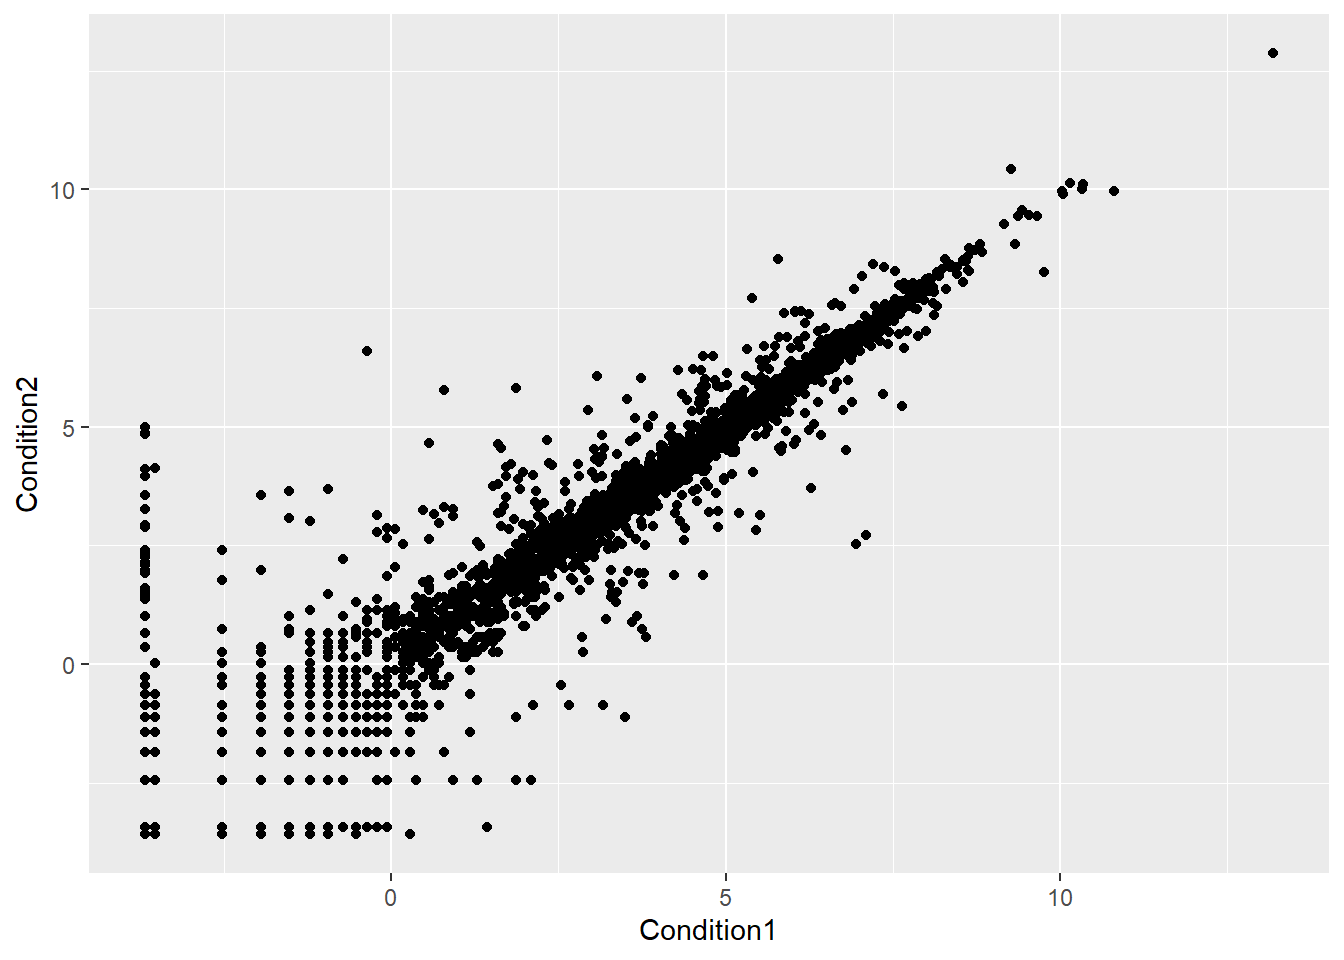
\includegraphics{class-13_files/figure-latex/unnamed-chunk-11-1.pdf}

\begin{Shaded}
\begin{Highlighting}[]
\NormalTok{meancounts}\SpecialCharTok{$}\NormalTok{log2fc }\OtherTok{\textless{}{-}} \FunctionTok{log2}\NormalTok{(meancounts[,}\StringTok{"treated.mean"}\NormalTok{]}\SpecialCharTok{/}\NormalTok{meancounts[,}\StringTok{"control.mean"}\NormalTok{])}
\FunctionTok{head}\NormalTok{(meancounts)}
\end{Highlighting}
\end{Shaded}

\begin{verbatim}
##                 control.mean treated.mean      log2fc
## ENSG00000000003       900.75       658.00 -0.45303916
## ENSG00000000005         0.00         0.00         NaN
## ENSG00000000419       520.50       546.00  0.06900279
## ENSG00000000457       339.75       316.50 -0.10226805
## ENSG00000000460        97.25        78.75 -0.30441833
## ENSG00000000938         0.75         0.00        -Inf
\end{verbatim}

\begin{Shaded}
\begin{Highlighting}[]
\NormalTok{zero.vals }\OtherTok{\textless{}{-}} \FunctionTok{which}\NormalTok{(meancounts[,}\DecValTok{1}\SpecialCharTok{:}\DecValTok{2}\NormalTok{]}\SpecialCharTok{==}\DecValTok{0}\NormalTok{, }\AttributeTok{arr.ind=}\ConstantTok{TRUE}\NormalTok{)}

\NormalTok{to.rm }\OtherTok{\textless{}{-}} \FunctionTok{unique}\NormalTok{(zero.vals[,}\DecValTok{1}\NormalTok{])}
\NormalTok{mycounts }\OtherTok{\textless{}{-}}\NormalTok{ meancounts[}\SpecialCharTok{{-}}\NormalTok{to.rm,]}
\FunctionTok{head}\NormalTok{(mycounts)}
\end{Highlighting}
\end{Shaded}

\begin{verbatim}
##                 control.mean treated.mean      log2fc
## ENSG00000000003       900.75       658.00 -0.45303916
## ENSG00000000419       520.50       546.00  0.06900279
## ENSG00000000457       339.75       316.50 -0.10226805
## ENSG00000000460        97.25        78.75 -0.30441833
## ENSG00000000971      5219.00      6687.50  0.35769358
## ENSG00000001036      2327.00      1785.75 -0.38194109
\end{verbatim}

\begin{quote}
Q7. What is the purpose of the arr.ind argument in the which() function
call above? Why would we then take the first column of the output and
need to call the unique() function?
\end{quote}

\begin{quote}
ANS: We are trying to get rid of zero count genes. The arr.ind argument
is used to find the array indices that contain 0.This allows us to know
which genes(rows) and samples(columns) contain 0.The unique() function
avoids duplication counting, especially if the samples of one gene have
two 0s.
\end{quote}

\begin{Shaded}
\begin{Highlighting}[]
\NormalTok{up.ind }\OtherTok{\textless{}{-}}\NormalTok{ mycounts}\SpecialCharTok{$}\NormalTok{log2fc }\SpecialCharTok{\textgreater{}} \DecValTok{2}
\NormalTok{down.ind }\OtherTok{\textless{}{-}}\NormalTok{ mycounts}\SpecialCharTok{$}\NormalTok{log2fc }\SpecialCharTok{\textless{}}\NormalTok{ (}\SpecialCharTok{{-}}\DecValTok{2}\NormalTok{)}
\end{Highlighting}
\end{Shaded}

\begin{quote}
Q8. Using the up.ind vector above can you determine how many up
regulated genes we have at the greater than 2 fc level? ANS:250
\end{quote}

\begin{Shaded}
\begin{Highlighting}[]
\FunctionTok{sum}\NormalTok{(up.ind)}
\end{Highlighting}
\end{Shaded}

\begin{verbatim}
## [1] 250
\end{verbatim}

\begin{quote}
Q9. Using the down.ind vector above can you determine how many down
regulated genes we have at the greater than 2 fc level? ANS:367
\end{quote}

\begin{Shaded}
\begin{Highlighting}[]
\FunctionTok{sum}\NormalTok{(down.ind)}
\end{Highlighting}
\end{Shaded}

\begin{verbatim}
## [1] 367
\end{verbatim}

\begin{quote}
Q10. Do you trust these results? Why or why not?
\end{quote}

\begin{quote}
Ans:No, I don't trust these results. The fold change of 2 is arbituary.
There is no statistical basis to its significance.
\end{quote}

\begin{Shaded}
\begin{Highlighting}[]
\FunctionTok{library}\NormalTok{(DESeq2)}
\end{Highlighting}
\end{Shaded}

\begin{verbatim}
## 载入需要的程序包:S4Vectors
\end{verbatim}

\begin{verbatim}
## 载入需要的程序包:stats4
\end{verbatim}

\begin{verbatim}
## 载入需要的程序包:BiocGenerics
\end{verbatim}

\begin{verbatim}
## 
## 载入程序包:'BiocGenerics'
\end{verbatim}

\begin{verbatim}
## The following objects are masked from 'package:stats':
## 
##     IQR, mad, sd, var, xtabs
\end{verbatim}

\begin{verbatim}
## The following objects are masked from 'package:base':
## 
##     anyDuplicated, aperm, append, as.data.frame, basename, cbind,
##     colnames, dirname, do.call, duplicated, eval, evalq, Filter, Find,
##     get, grep, grepl, intersect, is.unsorted, lapply, Map, mapply,
##     match, mget, order, paste, pmax, pmax.int, pmin, pmin.int,
##     Position, rank, rbind, Reduce, rownames, sapply, saveRDS, setdiff,
##     table, tapply, union, unique, unsplit, which.max, which.min
\end{verbatim}

\begin{verbatim}
## 
## 载入程序包:'S4Vectors'
\end{verbatim}

\begin{verbatim}
## The following object is masked from 'package:utils':
## 
##     findMatches
\end{verbatim}

\begin{verbatim}
## The following objects are masked from 'package:base':
## 
##     expand.grid, I, unname
\end{verbatim}

\begin{verbatim}
## 载入需要的程序包:IRanges
\end{verbatim}

\begin{verbatim}
## 
## 载入程序包:'IRanges'
\end{verbatim}

\begin{verbatim}
## The following object is masked from 'package:grDevices':
## 
##     windows
\end{verbatim}

\begin{verbatim}
## 载入需要的程序包:GenomicRanges
\end{verbatim}

\begin{verbatim}
## 载入需要的程序包:GenomeInfoDb
\end{verbatim}

\begin{verbatim}
## 载入需要的程序包:SummarizedExperiment
\end{verbatim}

\begin{verbatim}
## 载入需要的程序包:MatrixGenerics
\end{verbatim}

\begin{verbatim}
## 载入需要的程序包:matrixStats
\end{verbatim}

\begin{verbatim}
## Warning: 程序包'matrixStats'是用R版本4.4.2 来建造的
\end{verbatim}

\begin{verbatim}
## 
## 载入程序包:'MatrixGenerics'
\end{verbatim}

\begin{verbatim}
## The following objects are masked from 'package:matrixStats':
## 
##     colAlls, colAnyNAs, colAnys, colAvgsPerRowSet, colCollapse,
##     colCounts, colCummaxs, colCummins, colCumprods, colCumsums,
##     colDiffs, colIQRDiffs, colIQRs, colLogSumExps, colMadDiffs,
##     colMads, colMaxs, colMeans2, colMedians, colMins, colOrderStats,
##     colProds, colQuantiles, colRanges, colRanks, colSdDiffs, colSds,
##     colSums2, colTabulates, colVarDiffs, colVars, colWeightedMads,
##     colWeightedMeans, colWeightedMedians, colWeightedSds,
##     colWeightedVars, rowAlls, rowAnyNAs, rowAnys, rowAvgsPerColSet,
##     rowCollapse, rowCounts, rowCummaxs, rowCummins, rowCumprods,
##     rowCumsums, rowDiffs, rowIQRDiffs, rowIQRs, rowLogSumExps,
##     rowMadDiffs, rowMads, rowMaxs, rowMeans2, rowMedians, rowMins,
##     rowOrderStats, rowProds, rowQuantiles, rowRanges, rowRanks,
##     rowSdDiffs, rowSds, rowSums2, rowTabulates, rowVarDiffs, rowVars,
##     rowWeightedMads, rowWeightedMeans, rowWeightedMedians,
##     rowWeightedSds, rowWeightedVars
\end{verbatim}

\begin{verbatim}
## 载入需要的程序包:Biobase
\end{verbatim}

\begin{verbatim}
## Welcome to Bioconductor
## 
##     Vignettes contain introductory material; view with
##     'browseVignettes()'. To cite Bioconductor, see
##     'citation("Biobase")', and for packages 'citation("pkgname")'.
\end{verbatim}

\begin{verbatim}
## 
## 载入程序包:'Biobase'
\end{verbatim}

\begin{verbatim}
## The following object is masked from 'package:MatrixGenerics':
## 
##     rowMedians
\end{verbatim}

\begin{verbatim}
## The following objects are masked from 'package:matrixStats':
## 
##     anyMissing, rowMedians
\end{verbatim}

\begin{Shaded}
\begin{Highlighting}[]
\FunctionTok{citation}\NormalTok{(}\StringTok{"DESeq2"}\NormalTok{)}
\end{Highlighting}
\end{Shaded}

\begin{verbatim}
## 在出版物中使用程序包时引用'DESeq2':
## 
##   Love, M.I., Huber, W., Anders, S. Moderated estimation of fold change
##   and dispersion for RNA-seq data with DESeq2 Genome Biology 15(12):550
##   (2014)
## 
## LaTeX的用户的BibTeX条目是
## 
##   @Article{,
##     title = {Moderated estimation of fold change and dispersion for RNA-seq data with DESeq2},
##     author = {Michael I. Love and Wolfgang Huber and Simon Anders},
##     year = {2014},
##     journal = {Genome Biology},
##     doi = {10.1186/s13059-014-0550-8},
##     volume = {15},
##     issue = {12},
##     pages = {550},
##   }
\end{verbatim}

\begin{Shaded}
\begin{Highlighting}[]
\NormalTok{dds }\OtherTok{\textless{}{-}} \FunctionTok{DESeqDataSetFromMatrix}\NormalTok{(}\AttributeTok{countData=}\NormalTok{counts, }
                              \AttributeTok{colData=}\NormalTok{metadata, }
                              \AttributeTok{design=}\SpecialCharTok{\textasciitilde{}}\NormalTok{dex)}
\end{Highlighting}
\end{Shaded}

\begin{verbatim}
## converting counts to integer mode
\end{verbatim}

\begin{verbatim}
## Warning in DESeqDataSet(se, design = design, ignoreRank): some variables in
## design formula are characters, converting to factors
\end{verbatim}

\begin{Shaded}
\begin{Highlighting}[]
\NormalTok{dds}
\end{Highlighting}
\end{Shaded}

\begin{verbatim}
## class: DESeqDataSet 
## dim: 38694 8 
## metadata(1): version
## assays(1): counts
## rownames(38694): ENSG00000000003 ENSG00000000005 ... ENSG00000283120
##   ENSG00000283123
## rowData names(0):
## colnames(8): SRR1039508 SRR1039509 ... SRR1039520 SRR1039521
## colData names(4): id dex celltype geo_id
\end{verbatim}

\begin{Shaded}
\begin{Highlighting}[]
\NormalTok{vsd }\OtherTok{\textless{}{-}} \FunctionTok{vst}\NormalTok{(dds, }\AttributeTok{blind =} \ConstantTok{FALSE}\NormalTok{)}
\FunctionTok{plotPCA}\NormalTok{(vsd, }\AttributeTok{intgroup =} \FunctionTok{c}\NormalTok{(}\StringTok{"dex"}\NormalTok{))}
\end{Highlighting}
\end{Shaded}

\begin{verbatim}
## using ntop=500 top features by variance
\end{verbatim}

\includegraphics{class-13_files/figure-latex/unnamed-chunk-19-1.pdf}

\begin{Shaded}
\begin{Highlighting}[]
\NormalTok{pcaData }\OtherTok{\textless{}{-}} \FunctionTok{plotPCA}\NormalTok{(vsd, }\AttributeTok{intgroup=}\FunctionTok{c}\NormalTok{(}\StringTok{"dex"}\NormalTok{), }\AttributeTok{returnData=}\ConstantTok{TRUE}\NormalTok{)}
\end{Highlighting}
\end{Shaded}

\begin{verbatim}
## using ntop=500 top features by variance
\end{verbatim}

\begin{Shaded}
\begin{Highlighting}[]
\FunctionTok{head}\NormalTok{(pcaData)}
\end{Highlighting}
\end{Shaded}

\begin{verbatim}
##                   PC1        PC2   group     dex       name
## SRR1039508 -17.607922 -10.225252 control control SRR1039508
## SRR1039509   4.996738  -7.238117 treated treated SRR1039509
## SRR1039512  -5.474456  -8.113993 control control SRR1039512
## SRR1039513  18.912974  -6.226041 treated treated SRR1039513
## SRR1039516 -14.729173  16.252000 control control SRR1039516
## SRR1039517   7.279863  21.008034 treated treated SRR1039517
\end{verbatim}

\begin{Shaded}
\begin{Highlighting}[]
\CommentTok{\# Calculate percent variance per PC for the plot axis labels}
\NormalTok{percentVar }\OtherTok{\textless{}{-}} \FunctionTok{round}\NormalTok{(}\DecValTok{100} \SpecialCharTok{*} \FunctionTok{attr}\NormalTok{(pcaData, }\StringTok{"percentVar"}\NormalTok{))}
\end{Highlighting}
\end{Shaded}

\begin{Shaded}
\begin{Highlighting}[]
\FunctionTok{ggplot}\NormalTok{(pcaData) }\SpecialCharTok{+}
  \FunctionTok{aes}\NormalTok{(}\AttributeTok{x =}\NormalTok{ PC1, }\AttributeTok{y =}\NormalTok{ PC2, }\AttributeTok{color =}\NormalTok{ dex) }\SpecialCharTok{+}
  \FunctionTok{geom\_point}\NormalTok{(}\AttributeTok{size =}\DecValTok{3}\NormalTok{) }\SpecialCharTok{+}
  \FunctionTok{xlab}\NormalTok{(}\FunctionTok{paste0}\NormalTok{(}\StringTok{"PC1: "}\NormalTok{, percentVar[}\DecValTok{1}\NormalTok{], }\StringTok{"\% variance"}\NormalTok{)) }\SpecialCharTok{+}
  \FunctionTok{ylab}\NormalTok{(}\FunctionTok{paste0}\NormalTok{(}\StringTok{"PC2: "}\NormalTok{, percentVar[}\DecValTok{2}\NormalTok{], }\StringTok{"\% variance"}\NormalTok{)) }\SpecialCharTok{+}
  \FunctionTok{coord\_fixed}\NormalTok{() }\SpecialCharTok{+}\FunctionTok{theme\_bw}\NormalTok{()}
\end{Highlighting}
\end{Shaded}

\includegraphics{class-13_files/figure-latex/unnamed-chunk-22-1.pdf}

\begin{Shaded}
\begin{Highlighting}[]
\NormalTok{dds }\OtherTok{\textless{}{-}} \FunctionTok{DESeq}\NormalTok{(dds)}
\end{Highlighting}
\end{Shaded}

\begin{verbatim}
## estimating size factors
\end{verbatim}

\begin{verbatim}
## estimating dispersions
\end{verbatim}

\begin{verbatim}
## gene-wise dispersion estimates
\end{verbatim}

\begin{verbatim}
## mean-dispersion relationship
\end{verbatim}

\begin{verbatim}
## final dispersion estimates
\end{verbatim}

\begin{verbatim}
## fitting model and testing
\end{verbatim}

\begin{Shaded}
\begin{Highlighting}[]
\NormalTok{res }\OtherTok{\textless{}{-}} \FunctionTok{results}\NormalTok{(dds)}
\NormalTok{res}
\end{Highlighting}
\end{Shaded}

\begin{verbatim}
## log2 fold change (MLE): dex treated vs control 
## Wald test p-value: dex treated vs control 
## DataFrame with 38694 rows and 6 columns
##                  baseMean log2FoldChange     lfcSE      stat    pvalue
##                 <numeric>      <numeric> <numeric> <numeric> <numeric>
## ENSG00000000003  747.1942     -0.3507030  0.168246 -2.084470 0.0371175
## ENSG00000000005    0.0000             NA        NA        NA        NA
## ENSG00000000419  520.1342      0.2061078  0.101059  2.039475 0.0414026
## ENSG00000000457  322.6648      0.0245269  0.145145  0.168982 0.8658106
## ENSG00000000460   87.6826     -0.1471420  0.257007 -0.572521 0.5669691
## ...                   ...            ...       ...       ...       ...
## ENSG00000283115  0.000000             NA        NA        NA        NA
## ENSG00000283116  0.000000             NA        NA        NA        NA
## ENSG00000283119  0.000000             NA        NA        NA        NA
## ENSG00000283120  0.974916      -0.668258   1.69456 -0.394354  0.693319
## ENSG00000283123  0.000000             NA        NA        NA        NA
##                      padj
##                 <numeric>
## ENSG00000000003  0.163035
## ENSG00000000005        NA
## ENSG00000000419  0.176032
## ENSG00000000457  0.961694
## ENSG00000000460  0.815849
## ...                   ...
## ENSG00000283115        NA
## ENSG00000283116        NA
## ENSG00000283119        NA
## ENSG00000283120        NA
## ENSG00000283123        NA
\end{verbatim}

\begin{Shaded}
\begin{Highlighting}[]
\NormalTok{res }\OtherTok{\textless{}{-}} \FunctionTok{results}\NormalTok{(dds)}
\NormalTok{res}
\end{Highlighting}
\end{Shaded}

\begin{verbatim}
## log2 fold change (MLE): dex treated vs control 
## Wald test p-value: dex treated vs control 
## DataFrame with 38694 rows and 6 columns
##                  baseMean log2FoldChange     lfcSE      stat    pvalue
##                 <numeric>      <numeric> <numeric> <numeric> <numeric>
## ENSG00000000003  747.1942     -0.3507030  0.168246 -2.084470 0.0371175
## ENSG00000000005    0.0000             NA        NA        NA        NA
## ENSG00000000419  520.1342      0.2061078  0.101059  2.039475 0.0414026
## ENSG00000000457  322.6648      0.0245269  0.145145  0.168982 0.8658106
## ENSG00000000460   87.6826     -0.1471420  0.257007 -0.572521 0.5669691
## ...                   ...            ...       ...       ...       ...
## ENSG00000283115  0.000000             NA        NA        NA        NA
## ENSG00000283116  0.000000             NA        NA        NA        NA
## ENSG00000283119  0.000000             NA        NA        NA        NA
## ENSG00000283120  0.974916      -0.668258   1.69456 -0.394354  0.693319
## ENSG00000283123  0.000000             NA        NA        NA        NA
##                      padj
##                 <numeric>
## ENSG00000000003  0.163035
## ENSG00000000005        NA
## ENSG00000000419  0.176032
## ENSG00000000457  0.961694
## ENSG00000000460  0.815849
## ...                   ...
## ENSG00000283115        NA
## ENSG00000283116        NA
## ENSG00000283119        NA
## ENSG00000283120        NA
## ENSG00000283123        NA
\end{verbatim}

\begin{Shaded}
\begin{Highlighting}[]
\NormalTok{res05 }\OtherTok{\textless{}{-}} \FunctionTok{results}\NormalTok{(dds, }\AttributeTok{alpha=}\FloatTok{0.05}\NormalTok{)}
\FunctionTok{summary}\NormalTok{(res05)}
\end{Highlighting}
\end{Shaded}

\begin{verbatim}
## 
## out of 25258 with nonzero total read count
## adjusted p-value < 0.05
## LFC > 0 (up)       : 1236, 4.9%
## LFC < 0 (down)     : 933, 3.7%
## outliers [1]       : 142, 0.56%
## low counts [2]     : 9033, 36%
## (mean count < 6)
## [1] see 'cooksCutoff' argument of ?results
## [2] see 'independentFiltering' argument of ?results
\end{verbatim}

\begin{Shaded}
\begin{Highlighting}[]
\FunctionTok{library}\NormalTok{(}\StringTok{"AnnotationDbi"}\NormalTok{)}
\FunctionTok{library}\NormalTok{(}\StringTok{"org.Hs.eg.db"}\NormalTok{)}
\end{Highlighting}
\end{Shaded}

\begin{verbatim}
## 
\end{verbatim}

\begin{Shaded}
\begin{Highlighting}[]
\FunctionTok{columns}\NormalTok{(org.Hs.eg.db)}
\end{Highlighting}
\end{Shaded}

\begin{verbatim}
##  [1] "ACCNUM"       "ALIAS"        "ENSEMBL"      "ENSEMBLPROT"  "ENSEMBLTRANS"
##  [6] "ENTREZID"     "ENZYME"       "EVIDENCE"     "EVIDENCEALL"  "GENENAME"    
## [11] "GENETYPE"     "GO"           "GOALL"        "IPI"          "MAP"         
## [16] "OMIM"         "ONTOLOGY"     "ONTOLOGYALL"  "PATH"         "PFAM"        
## [21] "PMID"         "PROSITE"      "REFSEQ"       "SYMBOL"       "UCSCKG"      
## [26] "UNIPROT"
\end{verbatim}

\begin{Shaded}
\begin{Highlighting}[]
\NormalTok{res}\SpecialCharTok{$}\NormalTok{symbol }\OtherTok{\textless{}{-}} \FunctionTok{mapIds}\NormalTok{(org.Hs.eg.db,}
                     \AttributeTok{keys=}\FunctionTok{row.names}\NormalTok{(res), }\CommentTok{\# Our genenames}
                     \AttributeTok{keytype=}\StringTok{"ENSEMBL"}\NormalTok{,        }\CommentTok{\# The format of our genenames}
                     \AttributeTok{column=}\StringTok{"SYMBOL"}\NormalTok{,          }\CommentTok{\# The new format we want to add}
                     \AttributeTok{multiVals=}\StringTok{"first"}\NormalTok{)}
\end{Highlighting}
\end{Shaded}

\begin{verbatim}
## 'select()' returned 1:many mapping between keys and columns
\end{verbatim}

\begin{Shaded}
\begin{Highlighting}[]
\FunctionTok{head}\NormalTok{(res)}
\end{Highlighting}
\end{Shaded}

\begin{verbatim}
## log2 fold change (MLE): dex treated vs control 
## Wald test p-value: dex treated vs control 
## DataFrame with 6 rows and 7 columns
##                   baseMean log2FoldChange     lfcSE      stat    pvalue
##                  <numeric>      <numeric> <numeric> <numeric> <numeric>
## ENSG00000000003 747.194195     -0.3507030  0.168246 -2.084470 0.0371175
## ENSG00000000005   0.000000             NA        NA        NA        NA
## ENSG00000000419 520.134160      0.2061078  0.101059  2.039475 0.0414026
## ENSG00000000457 322.664844      0.0245269  0.145145  0.168982 0.8658106
## ENSG00000000460  87.682625     -0.1471420  0.257007 -0.572521 0.5669691
## ENSG00000000938   0.319167     -1.7322890  3.493601 -0.495846 0.6200029
##                      padj      symbol
##                 <numeric> <character>
## ENSG00000000003  0.163035      TSPAN6
## ENSG00000000005        NA        TNMD
## ENSG00000000419  0.176032        DPM1
## ENSG00000000457  0.961694       SCYL3
## ENSG00000000460  0.815849       FIRRM
## ENSG00000000938        NA         FGR
\end{verbatim}

Q11. Run the mapIds() function two more times to add the Entrez ID and
UniProt accession and GENENAME as new columns called
res\(entrez, res\)uniprot and res\$genename.

\begin{Shaded}
\begin{Highlighting}[]
\NormalTok{res}\SpecialCharTok{$}\NormalTok{entrez }\OtherTok{\textless{}{-}} \FunctionTok{mapIds}\NormalTok{(org.Hs.eg.db,}
                     \AttributeTok{keys=}\FunctionTok{row.names}\NormalTok{(res),}
                     \AttributeTok{column=}\StringTok{"ENTREZID"}\NormalTok{,}
                     \AttributeTok{keytype=}\StringTok{"ENSEMBL"}\NormalTok{,}
                     \AttributeTok{multiVals=}\StringTok{"first"}\NormalTok{)}
\end{Highlighting}
\end{Shaded}

\begin{verbatim}
## 'select()' returned 1:many mapping between keys and columns
\end{verbatim}

\begin{Shaded}
\begin{Highlighting}[]
\NormalTok{res}\SpecialCharTok{$}\NormalTok{uniprot }\OtherTok{\textless{}{-}} \FunctionTok{mapIds}\NormalTok{(org.Hs.eg.db,}
                     \AttributeTok{keys=}\FunctionTok{row.names}\NormalTok{(res),}
                     \AttributeTok{column=}\StringTok{"UNIPROT"}\NormalTok{,}
                     \AttributeTok{keytype=}\StringTok{"ENSEMBL"}\NormalTok{,}
                     \AttributeTok{multiVals=}\StringTok{"first"}\NormalTok{)}
\end{Highlighting}
\end{Shaded}

\begin{verbatim}
## 'select()' returned 1:many mapping between keys and columns
\end{verbatim}

\begin{Shaded}
\begin{Highlighting}[]
\NormalTok{res}\SpecialCharTok{$}\NormalTok{genename }\OtherTok{\textless{}{-}} \FunctionTok{mapIds}\NormalTok{(org.Hs.eg.db,}
                     \AttributeTok{keys=}\FunctionTok{row.names}\NormalTok{(res),}
                     \AttributeTok{column=}\StringTok{"GENENAME"}\NormalTok{,}
                     \AttributeTok{keytype=}\StringTok{"ENSEMBL"}\NormalTok{,}
                     \AttributeTok{multiVals=}\StringTok{"first"}\NormalTok{)}
\end{Highlighting}
\end{Shaded}

\begin{verbatim}
## 'select()' returned 1:many mapping between keys and columns
\end{verbatim}

\begin{Shaded}
\begin{Highlighting}[]
\FunctionTok{head}\NormalTok{(res)}
\end{Highlighting}
\end{Shaded}

\begin{verbatim}
## log2 fold change (MLE): dex treated vs control 
## Wald test p-value: dex treated vs control 
## DataFrame with 6 rows and 10 columns
##                   baseMean log2FoldChange     lfcSE      stat    pvalue
##                  <numeric>      <numeric> <numeric> <numeric> <numeric>
## ENSG00000000003 747.194195     -0.3507030  0.168246 -2.084470 0.0371175
## ENSG00000000005   0.000000             NA        NA        NA        NA
## ENSG00000000419 520.134160      0.2061078  0.101059  2.039475 0.0414026
## ENSG00000000457 322.664844      0.0245269  0.145145  0.168982 0.8658106
## ENSG00000000460  87.682625     -0.1471420  0.257007 -0.572521 0.5669691
## ENSG00000000938   0.319167     -1.7322890  3.493601 -0.495846 0.6200029
##                      padj      symbol      entrez     uniprot
##                 <numeric> <character> <character> <character>
## ENSG00000000003  0.163035      TSPAN6        7105  A0A087WYV6
## ENSG00000000005        NA        TNMD       64102      Q9H2S6
## ENSG00000000419  0.176032        DPM1        8813      H0Y368
## ENSG00000000457  0.961694       SCYL3       57147      X6RHX1
## ENSG00000000460  0.815849       FIRRM       55732      A6NFP1
## ENSG00000000938        NA         FGR        2268      B7Z6W7
##                               genename
##                            <character>
## ENSG00000000003          tetraspanin 6
## ENSG00000000005            tenomodulin
## ENSG00000000419 dolichyl-phosphate m..
## ENSG00000000457 SCY1 like pseudokina..
## ENSG00000000460 FIGNL1 interacting r..
## ENSG00000000938 FGR proto-oncogene, ..
\end{verbatim}

\begin{Shaded}
\begin{Highlighting}[]
\NormalTok{ord }\OtherTok{\textless{}{-}} \FunctionTok{order}\NormalTok{( res}\SpecialCharTok{$}\NormalTok{padj )}
\CommentTok{\#View(res[ord,])}
\FunctionTok{head}\NormalTok{(res[ord,])}
\end{Highlighting}
\end{Shaded}

\begin{verbatim}
## log2 fold change (MLE): dex treated vs control 
## Wald test p-value: dex treated vs control 
## DataFrame with 6 rows and 10 columns
##                  baseMean log2FoldChange     lfcSE      stat      pvalue
##                 <numeric>      <numeric> <numeric> <numeric>   <numeric>
## ENSG00000152583   954.771        4.36836 0.2371268   18.4220 8.74490e-76
## ENSG00000179094   743.253        2.86389 0.1755693   16.3120 8.10784e-60
## ENSG00000116584  2277.913       -1.03470 0.0650984  -15.8944 6.92855e-57
## ENSG00000189221  2383.754        3.34154 0.2124058   15.7319 9.14433e-56
## ENSG00000120129  3440.704        2.96521 0.2036951   14.5571 5.26424e-48
## ENSG00000148175 13493.920        1.42717 0.1003890   14.2164 7.25128e-46
##                        padj      symbol      entrez     uniprot
##                   <numeric> <character> <character> <character>
## ENSG00000152583 1.32441e-71     SPARCL1        8404      B4E2Z0
## ENSG00000179094 6.13966e-56        PER1        5187      A2I2P6
## ENSG00000116584 3.49776e-53     ARHGEF2        9181  A0A8Q3SIN5
## ENSG00000189221 3.46227e-52        MAOA        4128      B4DF46
## ENSG00000120129 1.59454e-44       DUSP1        1843      B4DRR4
## ENSG00000148175 1.83034e-42        STOM        2040      F8VSL7
##                               genename
##                            <character>
## ENSG00000152583           SPARC like 1
## ENSG00000179094 period circadian reg..
## ENSG00000116584 Rho/Rac guanine nucl..
## ENSG00000189221    monoamine oxidase A
## ENSG00000120129 dual specificity pho..
## ENSG00000148175               stomatin
\end{verbatim}

\begin{Shaded}
\begin{Highlighting}[]
\FunctionTok{write.csv}\NormalTok{(res[ord,], }\StringTok{"deseq\_results.csv"}\NormalTok{)}
\end{Highlighting}
\end{Shaded}

\begin{Shaded}
\begin{Highlighting}[]
\FunctionTok{plot}\NormalTok{( res}\SpecialCharTok{$}\NormalTok{log2FoldChange,  }\SpecialCharTok{{-}}\FunctionTok{log}\NormalTok{(res}\SpecialCharTok{$}\NormalTok{padj), }
      \AttributeTok{xlab=}\StringTok{"Log2(FoldChange)"}\NormalTok{,}
      \AttributeTok{ylab=}\StringTok{"{-}Log(P{-}value)"}\NormalTok{)}
\end{Highlighting}
\end{Shaded}

\includegraphics{class-13_files/figure-latex/unnamed-chunk-34-1.pdf}

\begin{Shaded}
\begin{Highlighting}[]
\FunctionTok{plot}\NormalTok{( res}\SpecialCharTok{$}\NormalTok{log2FoldChange,  }\SpecialCharTok{{-}}\FunctionTok{log}\NormalTok{(res}\SpecialCharTok{$}\NormalTok{padj), }
 \AttributeTok{ylab=}\StringTok{"{-}Log(P{-}value)"}\NormalTok{, }\AttributeTok{xlab=}\StringTok{"Log2(FoldChange)"}\NormalTok{)}

\CommentTok{\# Add some cut{-}off lines}
\FunctionTok{abline}\NormalTok{(}\AttributeTok{v=}\FunctionTok{c}\NormalTok{(}\SpecialCharTok{{-}}\DecValTok{2}\NormalTok{,}\DecValTok{2}\NormalTok{), }\AttributeTok{col=}\StringTok{"darkgray"}\NormalTok{, }\AttributeTok{lty=}\DecValTok{2}\NormalTok{)}
\FunctionTok{abline}\NormalTok{(}\AttributeTok{h=}\SpecialCharTok{{-}}\FunctionTok{log}\NormalTok{(}\FloatTok{0.05}\NormalTok{), }\AttributeTok{col=}\StringTok{"darkgray"}\NormalTok{, }\AttributeTok{lty=}\DecValTok{2}\NormalTok{)}
\end{Highlighting}
\end{Shaded}

\includegraphics{class-13_files/figure-latex/unnamed-chunk-35-1.pdf}

\begin{Shaded}
\begin{Highlighting}[]
\CommentTok{\# Setup our custom point color vector }
\NormalTok{mycols }\OtherTok{\textless{}{-}} \FunctionTok{rep}\NormalTok{(}\StringTok{"gray"}\NormalTok{, }\FunctionTok{nrow}\NormalTok{(res))}
\NormalTok{mycols[ }\FunctionTok{abs}\NormalTok{(res}\SpecialCharTok{$}\NormalTok{log2FoldChange) }\SpecialCharTok{\textgreater{}} \DecValTok{2}\NormalTok{ ]  }\OtherTok{\textless{}{-}} \StringTok{"red"} 

\NormalTok{inds }\OtherTok{\textless{}{-}}\NormalTok{ (res}\SpecialCharTok{$}\NormalTok{padj }\SpecialCharTok{\textless{}} \FloatTok{0.01}\NormalTok{) }\SpecialCharTok{\&}\NormalTok{ (}\FunctionTok{abs}\NormalTok{(res}\SpecialCharTok{$}\NormalTok{log2FoldChange) }\SpecialCharTok{\textgreater{}} \DecValTok{2}\NormalTok{ )}
\NormalTok{mycols[ inds ] }\OtherTok{\textless{}{-}} \StringTok{"blue"}

\CommentTok{\# Volcano plot with custom colors }
\FunctionTok{plot}\NormalTok{( res}\SpecialCharTok{$}\NormalTok{log2FoldChange,  }\SpecialCharTok{{-}}\FunctionTok{log}\NormalTok{(res}\SpecialCharTok{$}\NormalTok{padj), }
 \AttributeTok{col=}\NormalTok{mycols, }\AttributeTok{ylab=}\StringTok{"{-}Log(P{-}value)"}\NormalTok{, }\AttributeTok{xlab=}\StringTok{"Log2(FoldChange)"}\NormalTok{ )}

\CommentTok{\# Cut{-}off lines}
\FunctionTok{abline}\NormalTok{(}\AttributeTok{v=}\FunctionTok{c}\NormalTok{(}\SpecialCharTok{{-}}\DecValTok{2}\NormalTok{,}\DecValTok{2}\NormalTok{), }\AttributeTok{col=}\StringTok{"gray"}\NormalTok{, }\AttributeTok{lty=}\DecValTok{2}\NormalTok{)}
\FunctionTok{abline}\NormalTok{(}\AttributeTok{h=}\SpecialCharTok{{-}}\FunctionTok{log}\NormalTok{(}\FloatTok{0.1}\NormalTok{), }\AttributeTok{col=}\StringTok{"gray"}\NormalTok{, }\AttributeTok{lty=}\DecValTok{2}\NormalTok{)}
\end{Highlighting}
\end{Shaded}

\includegraphics{class-13_files/figure-latex/unnamed-chunk-36-1.pdf}
BiocManager::install(``EnhancedVolcano'')`

\begin{Shaded}
\begin{Highlighting}[]
\FunctionTok{library}\NormalTok{(EnhancedVolcano)}
\end{Highlighting}
\end{Shaded}

\begin{verbatim}
## 载入需要的程序包:ggrepel
\end{verbatim}

\begin{Shaded}
\begin{Highlighting}[]
\NormalTok{x }\OtherTok{\textless{}{-}} \FunctionTok{as.data.frame}\NormalTok{(res)}

\FunctionTok{EnhancedVolcano}\NormalTok{(x,}
    \AttributeTok{lab =}\NormalTok{ x}\SpecialCharTok{$}\NormalTok{symbol,}
    \AttributeTok{x =} \StringTok{\textquotesingle{}log2FoldChange\textquotesingle{}}\NormalTok{,}
    \AttributeTok{y =} \StringTok{\textquotesingle{}pvalue\textquotesingle{}}\NormalTok{)}
\end{Highlighting}
\end{Shaded}

\includegraphics{class-13_files/figure-latex/unnamed-chunk-38-1.pdf}

\end{document}
